\section{Gathering of Data}

I used the  \href{https://www.kaggle.com/Cornell-University/arxiv}{Arxiv} and Neural Information Processing 
    Systems (\href{https://www.kaggle.com/benhamner/nips-papers}{NIPS}) datasets from kaggle. On listing \ref{schemas}
we can see raw schema of the files. Arxiv in json format and NIPS is on csv files. I hosted both files on a S3: 
\emph{s3a://arxivs3/input\_data/arxiv-metadata-oai-snapshot.json}, \emph{s3a://arxivs3/input\_data/NIPS.csv}. To upload the
data to s3, I had to create an EC2 instance, install \emph{miniconda}, \emph{kaggle} library and aws client (see listing \ref{transfer}). 
   
\begin{mdframed}[backgroundcolor=light-gray, roundcorner=10pt,leftmargin=1, rightmargin=1, innerleftmargin=15, innertopmargin=15,innerbottommargin=15, outerlinewidth=1, linecolor=light-gray]
\begin{lstlisting}[caption={Datasets Schema},label={schemas}]    
>>> df_arxiv.printSchema()
root
 |-- abstract: string (nullable = true)
 |-- authors: string (nullable = true)
 |-- authors_parsed: array (nullable = true)
 |    |-- element: array (containsNull = true)
 |    |    |-- element: string (containsNull = true)
 |-- categories: string (nullable = true)
 |-- comments: string (nullable = true)
 |-- doi: string (nullable = true)
 |-- id: string (nullable = true)
 |-- journal-ref: string (nullable = true)
 |-- license: string (nullable = true)
 |-- report-no: string (nullable = true)
 |-- submitter: string (nullable = true)
 |-- title: string (nullable = true)
 |-- update_date: string (nullable = true)
 |-- versions: array (nullable = true)
 |    |-- element: struct (containsNull = true)
 |    |    |-- created: string (nullable = true)
 |    |    |-- version: string (nullable = true)
 
>>> df_papers_nips.printSchema()
root
 |-- id: string (nullable = true)
 |-- year: string (nullable = true)
 |-- title: string (nullable = true)
 |-- abstract: string (nullable = true)
\end{lstlisting}
\end{mdframed} 

\begin{mdframed}[backgroundcolor=light-gray, roundcorner=10pt,leftmargin=0, rightmargin=0, innerleftmargin=15, innertopmargin=15,innerbottommargin=15, outerlinewidth=0, linecolor=light-gray]
\begin{lstlisting}[caption={From kaggle to S3 file transfer.},label={transfer}] 
# on a EC2 instance, install miniconda
Wget https://repo.anaconda.com/miniconda/Miniconda3-latest-Linux-x86_64.sh
bash https://repo.anaconda.com/miniconda/Miniconda3-latest-Linux-x86_64.sh
source .bashrc

# install kaggle library
pip install kaggle

# provide your kaggle credentials and change security of file
chmod 600 ~/.kaggle/kaggle.json

# get the dataset
kaggle datasets download Cornell-University/arxiv

# install aws client
curl "https://awscli.amazonaws.com/awscli-exe-linux-x86_64.zip" -o "awscliv2.zip"
unzip awscliv2.zip
sudo ./aws/install

# copy EC2 file to s3
aws s3 cp ./arxiv-metadata-oai-snapshot.json s3://arxivs3/input_data/
\end{lstlisting}
\end{mdframed} 



\subsection{About ArXiv Dataset}
For nearly 30 years, ArXiv has served the public and research communities by providing open access to scholarly articles, from the vast branches of physics to the many subdisciplines of computer science to everything in between, including math, statistics, electrical engineering, quantitative biology, and economics. This rich corpus of information offers significant, but sometimes overwhelming depth.\\

In these times of unique global challenges, efficient extraction of insights from data is essential. To help make the arXiv more accessible, we present a free, open pipeline on Kaggle to the machine-readable arXiv dataset: a repository of 1.7 million articles, with relevant features such as article titles, authors, categories, abstracts, full text PDFs, and more.\\

Our hope is to empower new use cases that can lead to the exploration of richer machine learning techniques that combine multi-modal features towards applications like trend analysis, paper recommender engines, category prediction, co-citation networks, knowledge graph construction and semantic search interfaces.\\

ArXiv is a collaboratively funded, community-supported resource founded by Paul Ginsparg in 1991 and maintained and operated by Cornell University.\\

\subsection{About NIPS Dataset}
Neural Information Processing Systems (NIPS) is one of the top machine learning conferences in the world. It covers topics ranging from deep learning and computer vision to cognitive science and reinforcement learning.\\

This dataset includes the title, authors, abstracts, and extracted text for all NIPS papers to date (ranging from the first 1987 conference to the current 2016 conference). I've extracted the paper text from the raw PDF files and are releasing that both in CSV files and as a SQLite database\\

\section{Exploration}

On the web application under the \emph{EDA} tab, it is possible to plot the current tendency on paper volume per year, and a distribution
of the topics \footnote{The application will query redshift to get the current state}. We see that papers increment exponentially with years, and also that the most popular topics are computer science, Math and Physics. The popularity of topics is always the same, since 2000.


\begin{figure}
\centering
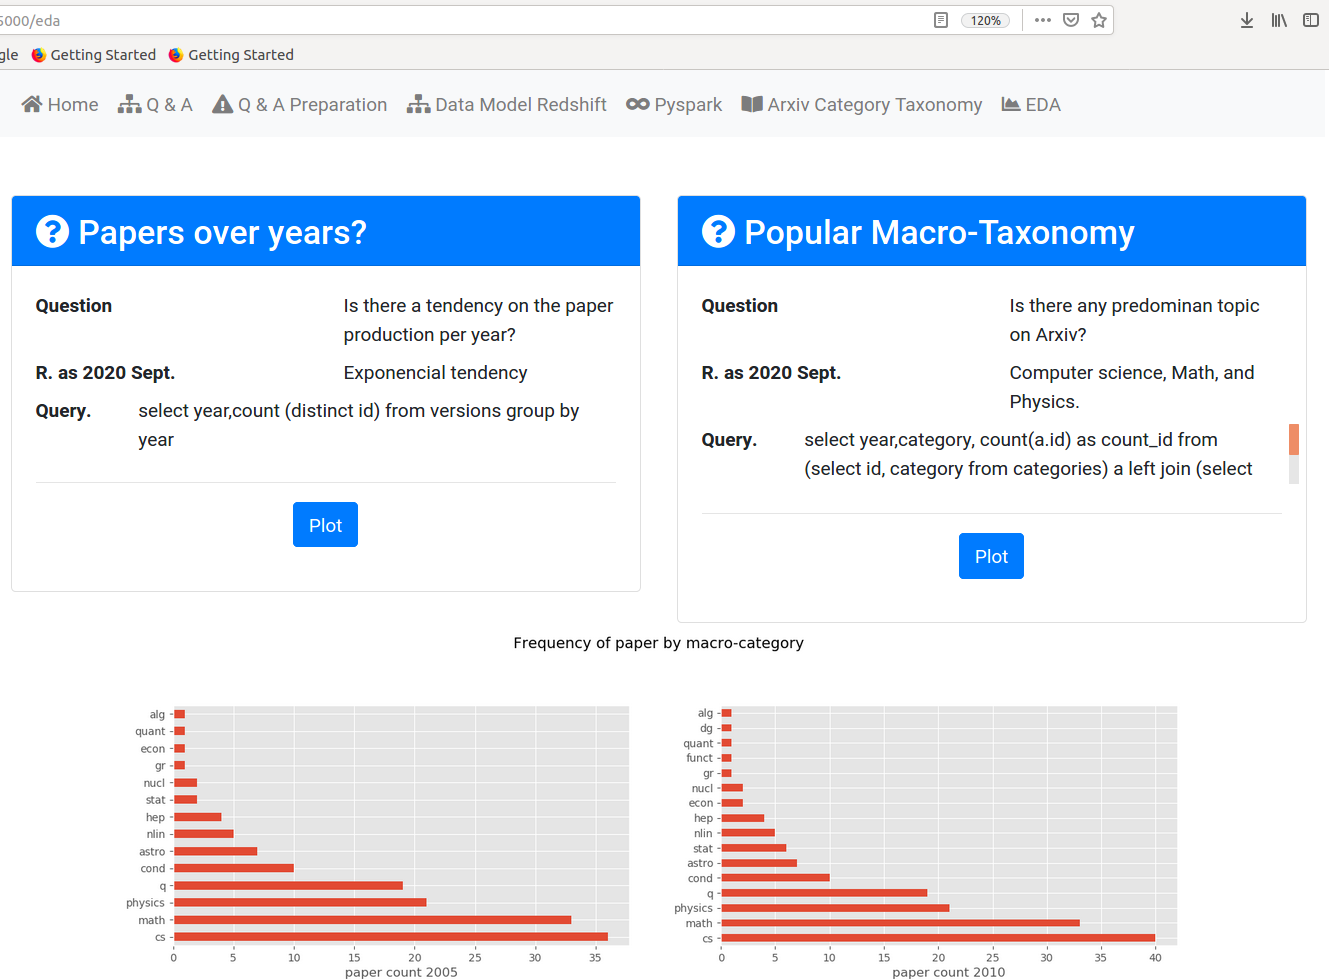
\includegraphics[width=1\linewidth]{images/4_eda}
\caption{Exploratory plots on Database.}
\label{fig:4_eda}
\end{figure}


\begin{figure}
\centering
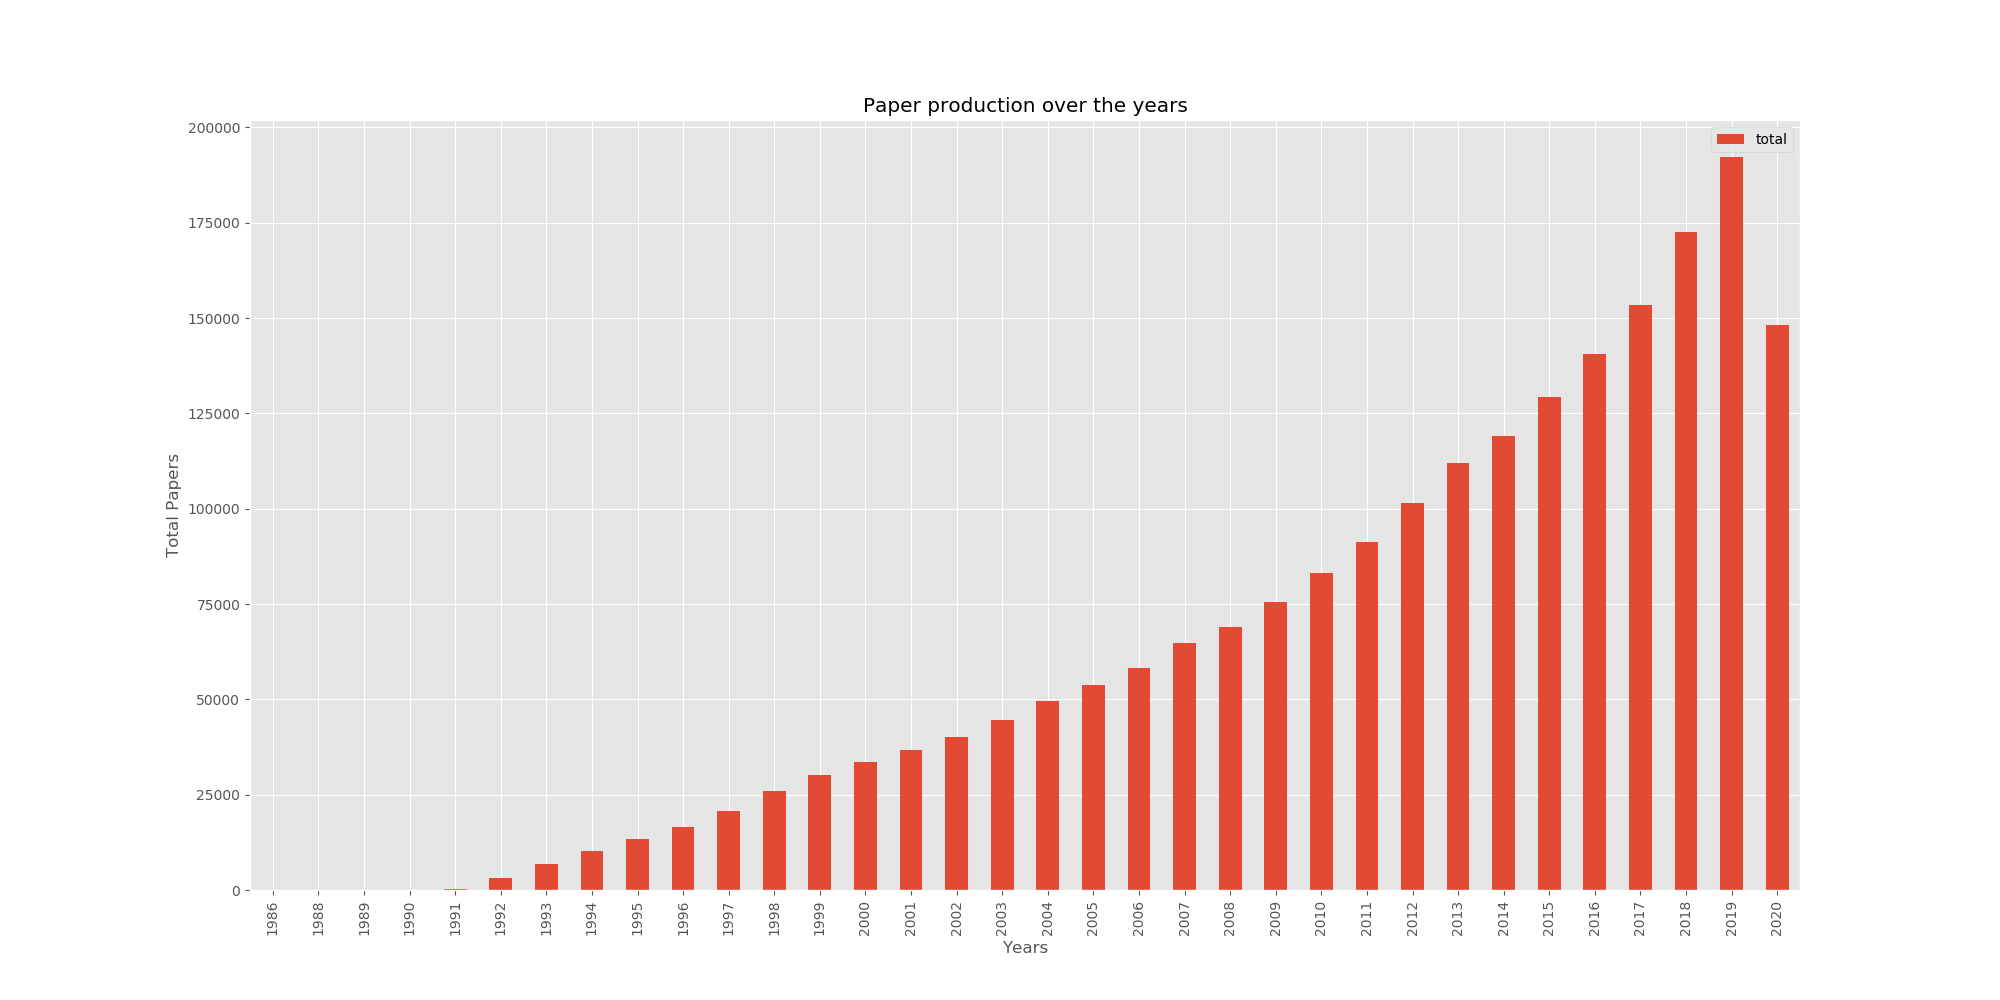
\includegraphics[width=1\linewidth]{images/paper_prod}
\caption{Paper production per year as Sept.2020}
\label{fig:paper_prod}
\end{figure}


\begin{figure}
\centering
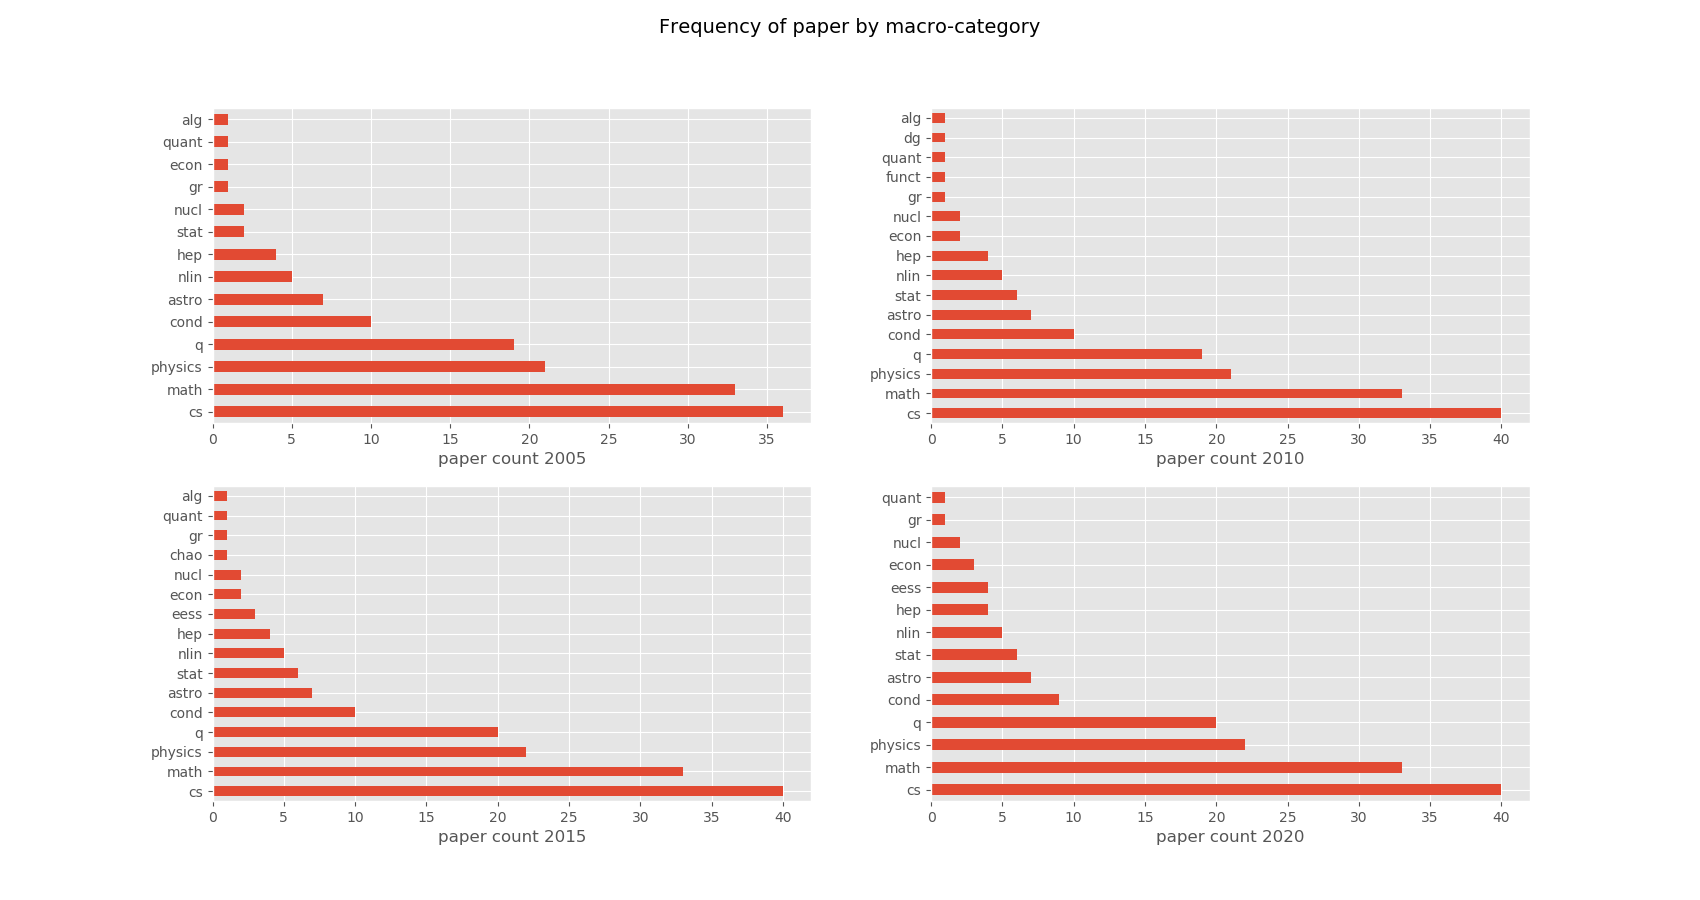
\includegraphics[width=1\linewidth]{images/paper_topics}
\caption{Popular topics in 2000 20010 2015 2020}
\label{fig:paper_topics}
\end{figure}

\subsection{Raw Volume and Uniqueness of the datasets.}

From listing \ref{vol} we can see that in ArXiv dataset there are 3 papers duplicated, whereas NIPS has none. On listing \ref{completeness}
we can observe that ArXiv contains 32982 rows completed informed, however we are more interested on the abstracts of the papers, and the id. 
By constraining the null statement, we now have 1753042 row informed. NIPS has all the row filled. 

\begin{mdframed}[backgroundcolor=light-gray, roundcorner=10pt,leftmargin=1, rightmargin=1, innerleftmargin=15, innertopmargin=15,innerbottommargin=15, outerlinewidth=1, linecolor=light-gray]
\begin{lstlisting}[caption={Volume and Uniqueness},label={vol}]  
>>> df_arxiv = spark.read.json(input_data_1)
>>> df_arxiv.persist()
>>> df_papers_nips = spark.read.format("csv")...
>>> df_arxiv.select("id").distinct().count()
1753039                                                                         
>>> df_arxiv.select("id").count()
1753042                                                                         
>>> df_papers_nips.select("id").distinct().count()
3946
>>> df_papers_nips.select("id").count()
3946
\end{lstlisting}
\end{mdframed} 

\begin{mdframed}[backgroundcolor=light-gray, roundcorner=10pt,leftmargin=1, rightmargin=1, innerleftmargin=15, innertopmargin=15,innerbottommargin=15, outerlinewidth=1, linecolor=light-gray]
\begin{lstlisting}[caption={Completeness of the Datastsets},label={completeness}]  
>>> df_arxiv.dropna().count()
32982                                                                           
>>> df_arxiv.dropna(subset=('id','abstract')).count()
1753042                                                                         
>>> df_papers_nips.dropna().count()
3924
\end{lstlisting}
\end{mdframed} 

\subsection{Assessment}
Since both data sets come from kaggle, they have great quality. Additionally, constraints on redshift enforce primary key uniqueness and nullity, so
no further quality checks were required.

\section{The Data model}

Initially, I thought having a star schema would be the correct choice. It would offer a degree of normalization, while still providing an easy to understand the data model. Nonetheless, upon trying to implement it, I realized that a query optimized model, where you have a table per query seems more appropriate, that way, in principle, you could train machine learning models per table, without having to refer to the fact table or others tables. On the other hand, I also envisioned non-technical users exploring basic trends, or asking questions about popular authors or topics in a given year. In the end, my data model resembles the star schema, allowing for ad hoc queries, while at the same time provides query optimized tables for machine learning. This hybrid approach was the main reason to select AWS Redshift cluster as the host of the model. Redshift provides Postgresql-like query language suitable for non-technical users while being Massively parallel processing (MPP) to operate on large amounts of Data. Additionally, Redshift is easily integrated with python3 with the \emph{psycopg2} module (for front-end) and with \emph{Airflow} through the Postgres operator.

\subsection{ETL}
Once I designed the data model and selected the hosting technology, I constructed the ETL scripts. I used \emph{PySpark} to transform the json and csv into DataFrames, process them and then leave them on S3 as parquet files. \emph{Spark}, in contrast to Redshift, supports json data manipulation, it is also parallelizable and comes with machine learning libraries. It is able to store data as parquet files, a columnar format particularity suitable for big data.\\

Most of the transformations involved flattening the nested data from the original .json, with the occasional use of regular expressions to extract temporal features of the records. All this process can be found in \href{https://github.com/gariciodaro/arXiv-haystack-app/blob/master/back_end/scripts/pysparkCreateParquets_TEMP.py}{pysparkCreateParquets\_TEMP.py}

\subsection{ETL Orchestration with Airflow}
\emph{Airflow} allows for ETL Orchestration with its webserver. I created tree Dags.  \href{https://github.com/gariciodaro/arXiv-haystack-app/blob/master/back_end/dags/createRedShiftDB.py}{create\_tables\_redshift} allows you to create the structure on Redshift of the data model. \href{https://github.com/gariciodaro/arXiv-haystack-app/blob/master/back_end/dags/sparkPreProcess.py}{create\_parquet\_area} runs \href{https://github.com/gariciodaro/arXiv-haystack-app/blob/master/back_end/scripts/pysparkCreateParquets_TEMP.py}{pysparkCreateParquets\_TEMP.py} script, and finally \href{https://github.com/gariciodaro/arXiv-haystack-app/blob/master/back_end/dags/RedShiftDataModel.py}{load\_data\_to\_redshift} copies the parquet files to Redshift and performs data quality checks (volumne checnk, and id nullity).\\

All the DAGs are set to run on demand, this means that a user would have to trigger the dag to actually execute it. If the user wanted to setup the automatic execution, for example \textbf{daily basis by 7am} all he/she needs to do is change the dag configurtaion (\emph{load\_data\_to\_redshift}) as in \ref{dag}.

\begin{mdframed}[backgroundcolor=light-gray, roundcorner=10pt,leftmargin=1, rightmargin=1, innerleftmargin=15, innertopmargin=15,innerbottommargin=15, outerlinewidth=1, linecolor=light-gray]
\begin{lstlisting}[caption={Dag configuration },label={dag}]  
args = {
    'owner': 'arXiv-haystack-app',
    'start_date': datetime.datetime.utcnow(),
    'catchup': False,
    'depends_on_past':False
}

dag = DAG(
        dag_id='create_parquet_area',
        default_args=args,
        schedule_interval='30 7 * * *')
        )
\end{lstlisting}
\end{mdframed} 

The whole development is ready to handle a 100x increase in data thanks to \emph{PySpark} scalability, and to withstand high user concurrency thanks to Redshift MPP nature.


\begin{figure}[h!]
\centering
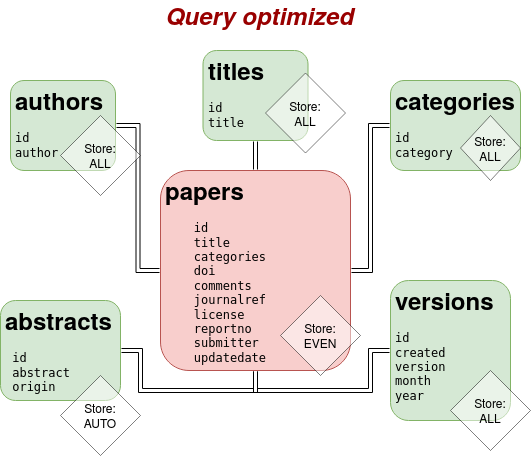
\includegraphics[width=0.4\linewidth]{images/star_schema}
\caption{Data model of Papers Data base}
\label{fig:star_schema}
\end{figure}

\section{front-end}
I used Flask to create a web interface that queries the redshifts back-end. My original idea was to allow the users to explore the database to select a subset of papers and then add the full-text paper to an elastic search cluster (key-pair document storage) for machine learning exploitation. Unfortunately the full pdfs of Arxiv are not available for \emph{wget} download, which I found out after finishing the code (can be seen on branch pdf\_fail\_aws). This pipeline consisted of obtaining the URL from Redshift, downloading the pdf to the client, and then upload them to s3, where Amazon Textract could process them asynchronously to text, and eventually append them to the local elastic search server. I was forced to change it to appending the title and abstract from Redshift to Elastic.


\begin{figure}
\centering
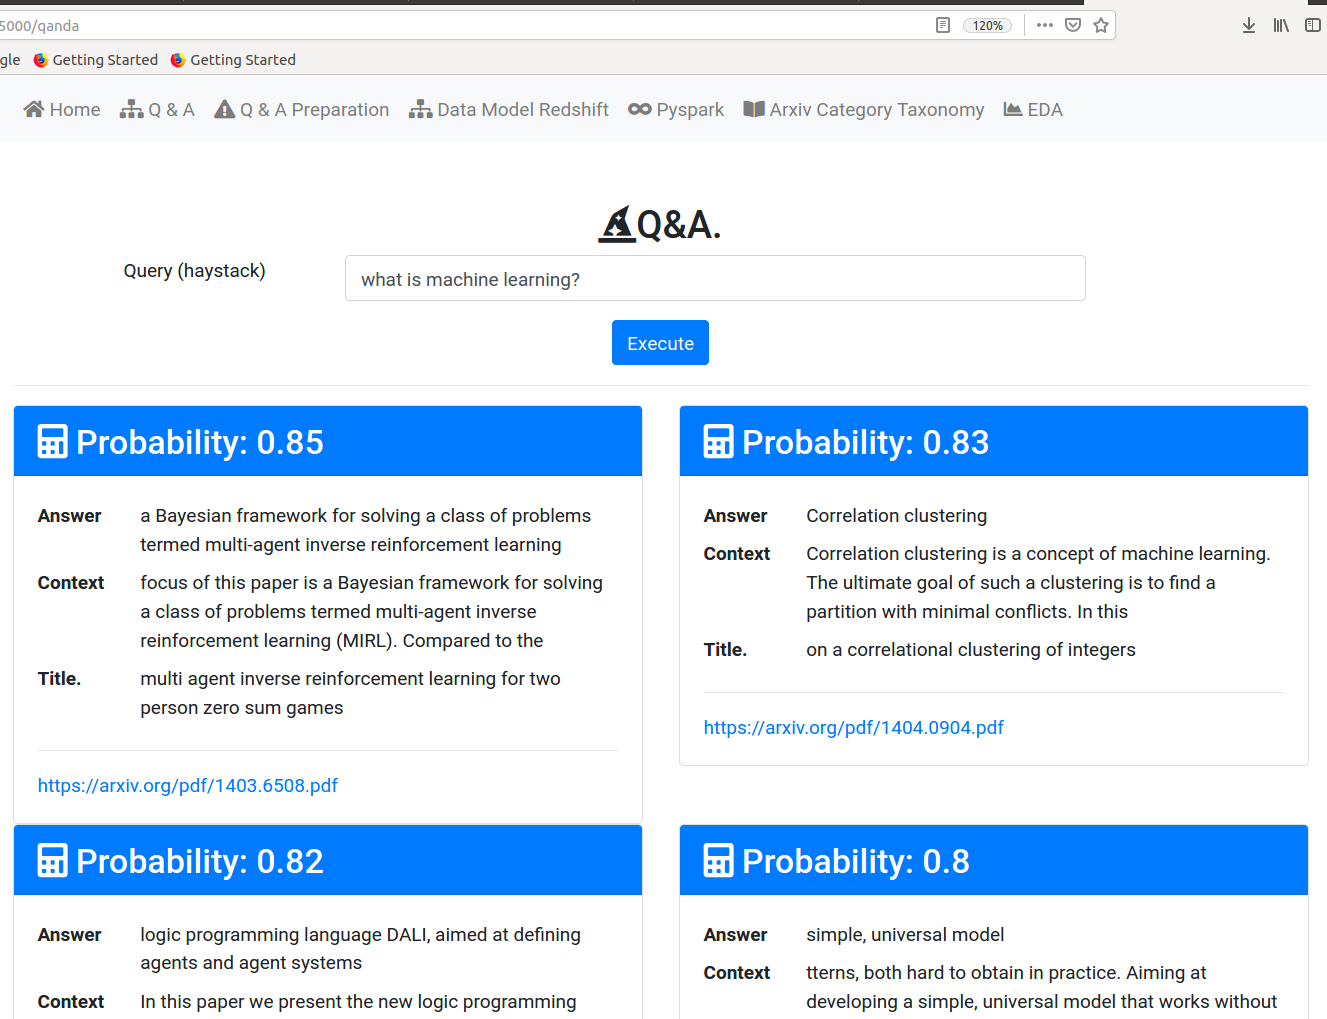
\includegraphics[width=0.9\linewidth]{images/3_make_questions}
\caption{Example of question and answers.}
\label{fig:3_make_questions}
\end{figure}


